\section{Introduction}
As part of the ongoing study of the structure of nucleons \cite{Avakian:2010ae}  in Hall B at the Thomas Jefferson National Accelerator Facility (JLab)  the CEBAF Large Acceptance Spectrometer (CLAS12) \cite{Burkert:2020akg} aims to accurately identify the secondary particles of high energy reactions, assist in probing the strangeness frontier, and aid in characterizing transverse momentum distribution (TMD) and generalized parton distribution (GPD) functions. Indispensable to this task is the ability to identify kaons, pions, and protons.  With the CLAS12 spectrometer providing accurate momentum measurements the Ring imagine Cherenkov detector (RICH) \cite{Contalbrigo:2020,Contalbrigo:2020snw,Mirazita:2017vav,Contalbrigo:2014rqa} provides tandem Cherenkov light-cone radius measurements which yield the velocities of near light-speed particles, thus facilitating mass-dependent particle identification.

\begin{figure}[hbt]
	\centering
	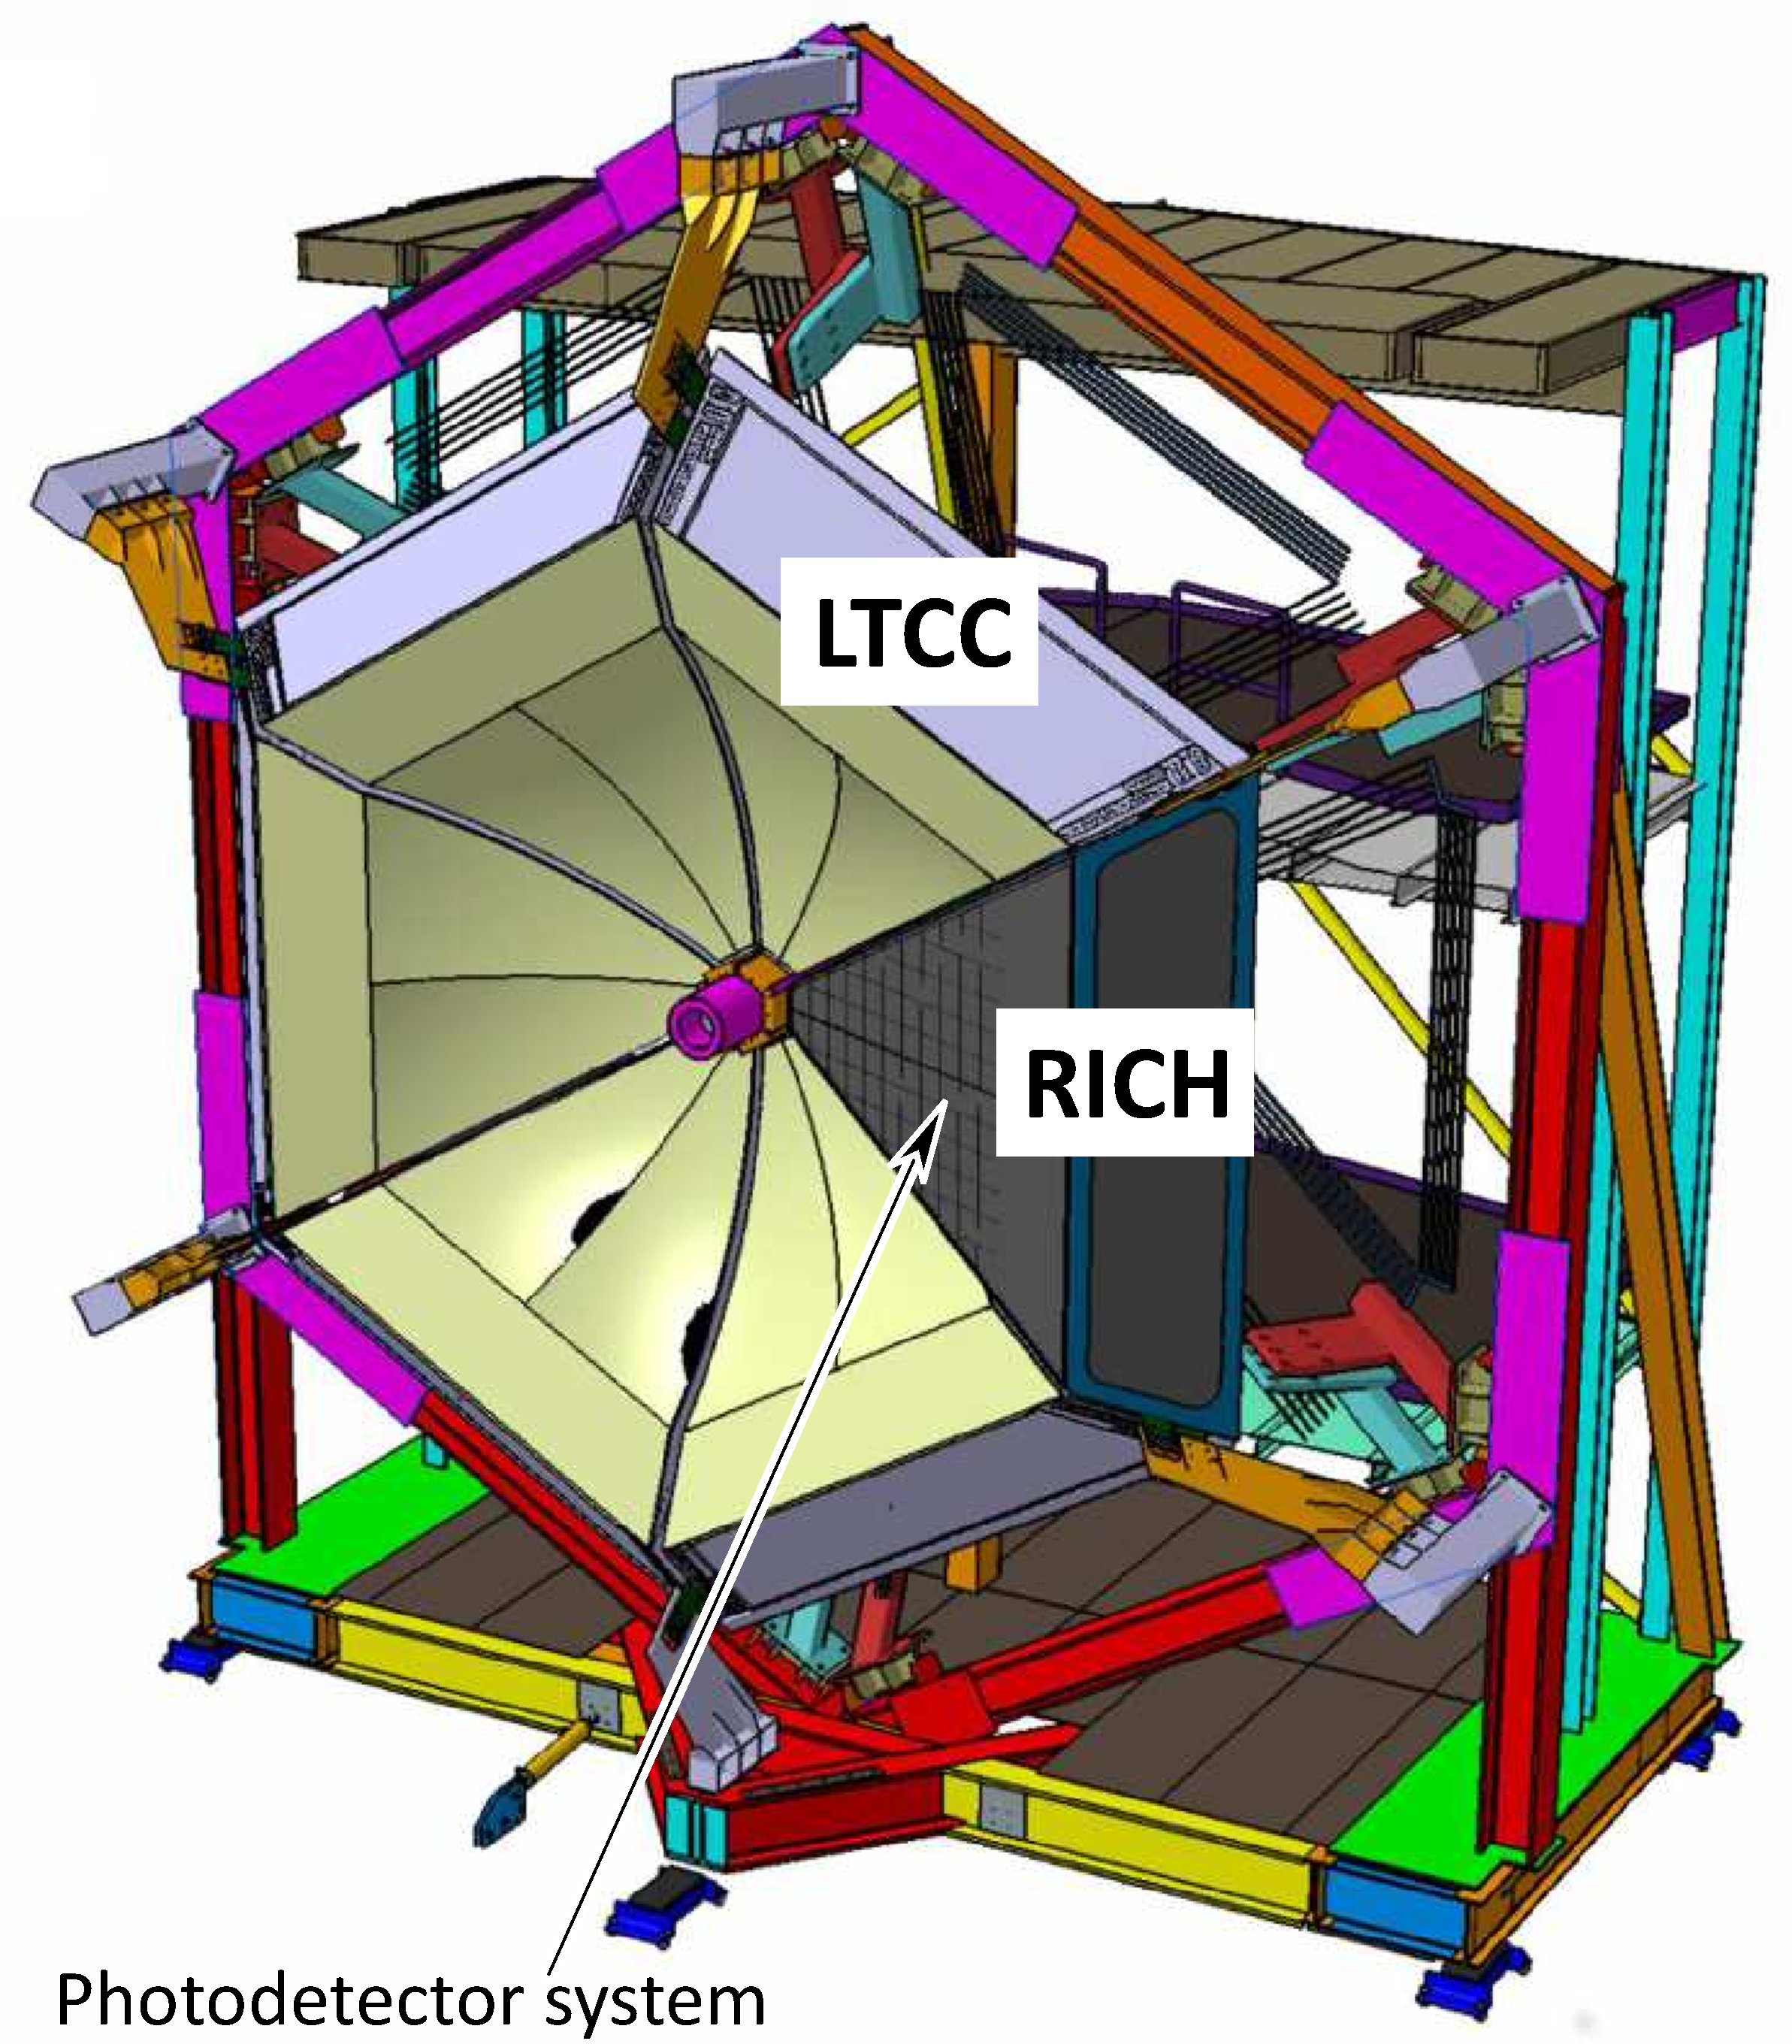
\includegraphics[width=0.7\linewidth]{figures/RICHdetector.pdf}
	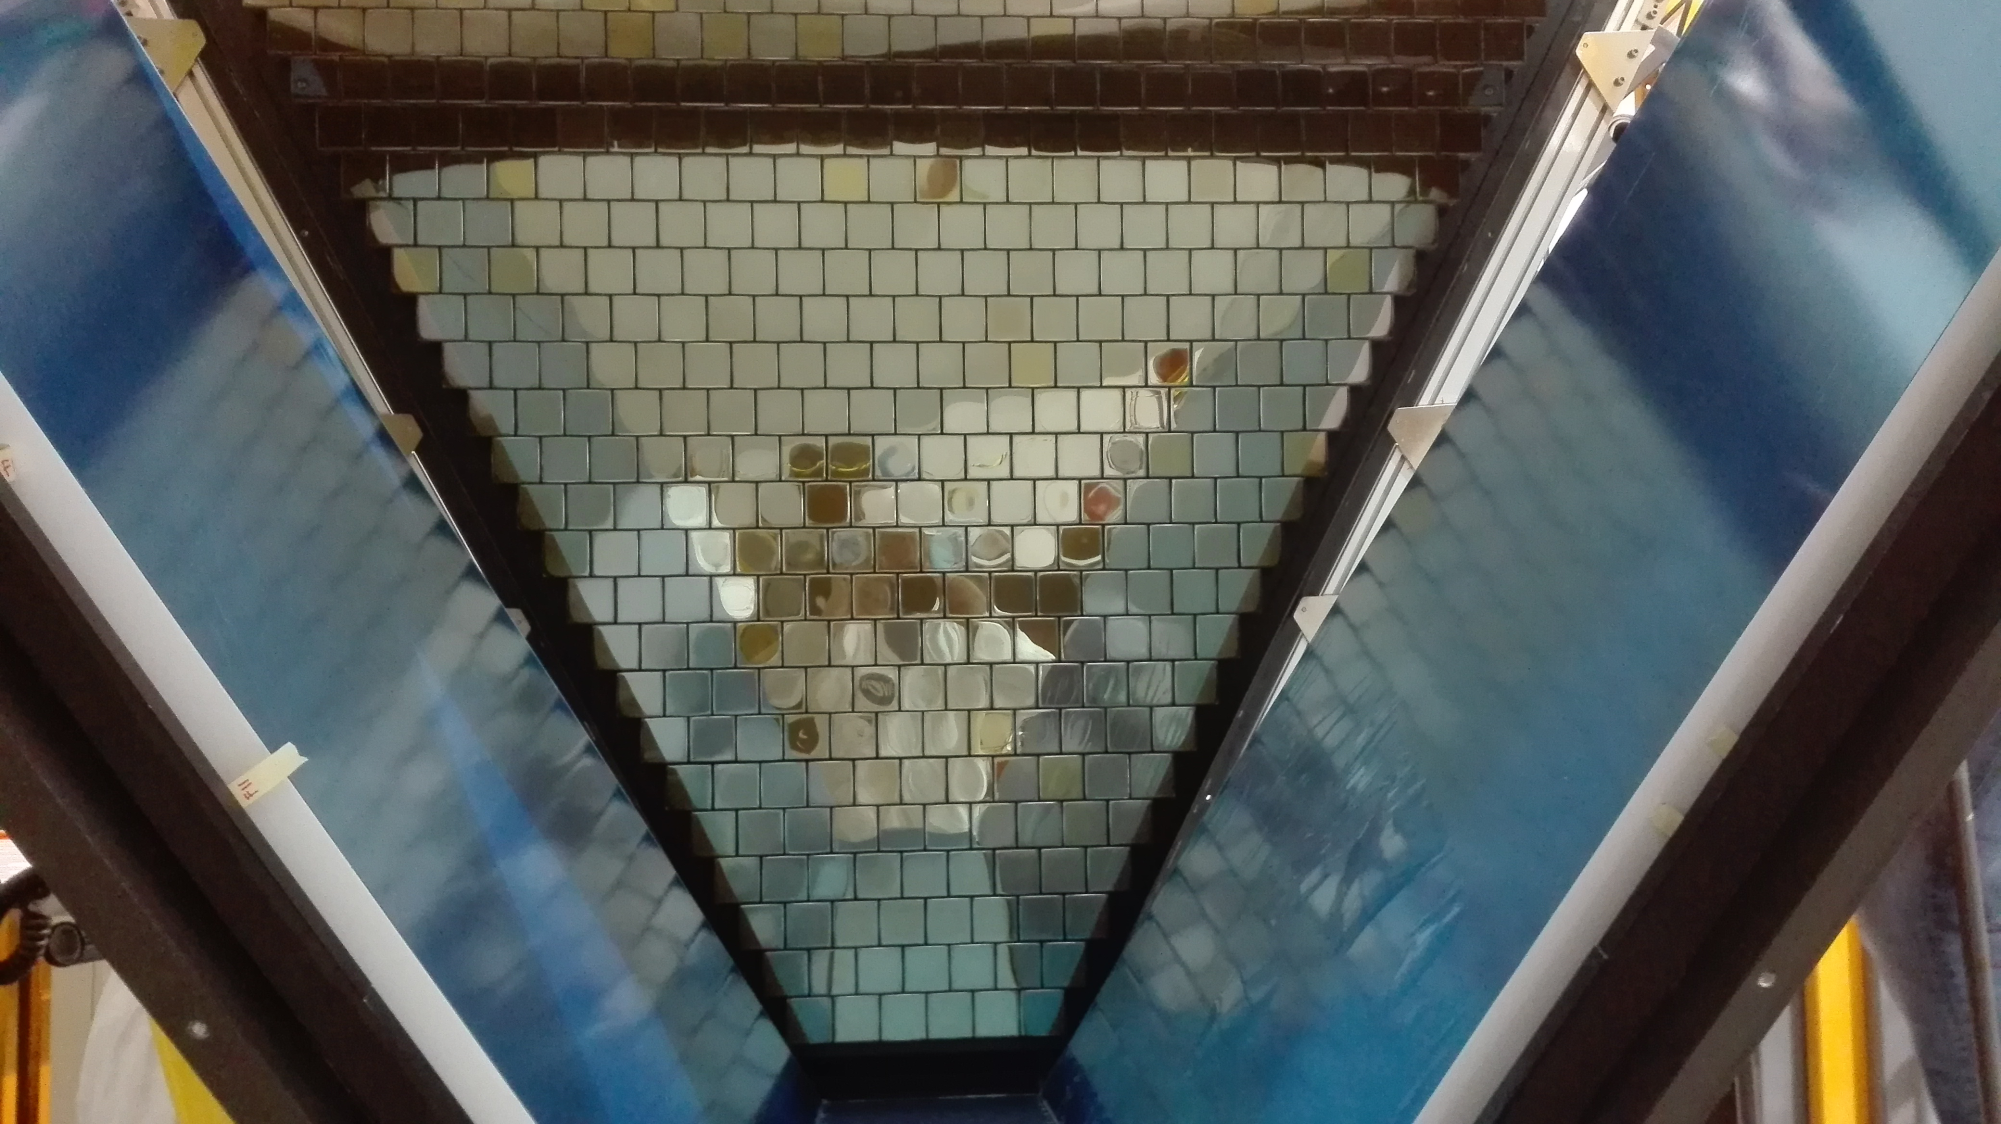
\includegraphics[width=0.7\linewidth]{figures/RICHpanel_front.png}
	\caption{Top: CLAS12 detector with RICH detector covering one out of six sectors. Bottom: the photo-matrix of multianode photomultipliers and mirror system.}
	\label{fig:RICHdetector}
\end{figure}

The photon detector wall ($\sim 1 m^2$) is a crucial component of the RICH detector (see Fig.~\ref{fig:RICHdetector}). It is relatively large and should be comprised of many photon detection devices such as photomultiplier tubes.
Due to the imaging aspect of the RICH they must provide a spatial resolution of less than 1 cm.
Since multiple photon detectors are tiled into large arrays, they should have large active area with minimal dead-space.
The photon detectors must also efficiently detect single photon level signals and should be sensitive to the visible light due to the aerogel radiator material.
Multi Anode PhotoMultiplier Tubes (MAPMTs) are perfect candidates for the CLAS12 RICH detector.
They are the flat-panel Hamamatsu MAPMTs offering an adequate compromise between detector performance and cost.
Each MAPMT comprises an 8 by 8 array of pixels, each with dimension of 6 by 6 mm.
Furthermore, the device has a very high packing fraction of 89\% with a high quantum efficiency in the visible light region.
The tubes also have excellent immunity to magnetic fields, because all internal parts are housed in a metal package and the distance between dynode electrodes are very short.


Initially, the Hamamatsu H8500 MAPMT model \cite{H8500} was chosen as the best option because they provide high quantum efficiency for visible light and sufficient spatial resolution (6x6 mm$^2$) at a limited cost.  However, recently Hamamatsu has released the new H12700 MAPMT model which shows enhanced single photoelectron (SPE) detection and is otherwise similar to the H8500 MAPMTs in spatial resolution and  cost.  Consequently we desire to better characterize the new H12700 MAPMTs \cite{H12700} and choose the best model between these two options for inclusion in the CLAS12 RICH.

